\documentclass[conference]{IEEEtran}
\usepackage{cite}
\usepackage{amsmath,amssymb,amsfonts}
\usepackage{algorithmic}
\usepackage{graphicx}
\usepackage{textcomp}
\usepackage{xcolor}
\def\BibTeX{{\rm B\kern-.05em{\sc i\kern-.025em b}\kern-.08em
    T\kern-.1667em\lower.7ex\hbox{E}\kern-.125emX}}
\begin{document}

\title{100W Low Voltage AC-DC Converter\\}


\author{\IEEEauthorblockN{Chasen Gaither}
\IEEEauthorblockA{\textit{Student ID: 1974745} \\
\textit{University of Washington}\\
Seattle, WA, USA \\
chasennn@uw.edu}
\and
\IEEEauthorblockN{Khushbu Patel}
\IEEEauthorblockA{\textit{Student ID: 2400367} \\
\textit{University of Washington}\\
Seattle, WA, USA \\
kbupatel@uw.edu}
\and
\IEEEauthorblockN{Enrique Antunano}
\IEEEauthorblockA{\textit{Student ID: 2400331} \\
\textit{University of Washington}\\
Seattle, WA, USA \\
enriantu@uw.edu}
}

\maketitle

\begin{abstract}
This document covers the design of a DO-160G EMI compliant AC-DC converter that accepts a 115 \textit{Vac}, 400 \textit{Hz}, voltage input
and can provide up to 100 \textit{W} to a 28 \textit{Vdc} output.
\end{abstract}

\section{Introduction}
This document covers the design of a DO-160G EMI compliant AC-DC converter that accepts a 115 \textit{Vac}, 400 \textit{Hz}, voltage input
and can provide up to 100 \textit{W} to a 28 \textit{Vdc} output. The power path will require AC rectification and a DC step-down with a buck converter. As the team's experience is in the aerospace industry, DO-160G EMI requirements will be used instead of FCC or CISPR requirements. DO-160G covers the compliance of aviation equipment in multiple environmental and electromagnetic conditions found in aircraft. DO-160G is referenced by the FAA’s Advisory Circular AC 21-16G and other regulatory authorities worldwide.

\section{Circuit Architecture}

\subsection{High-Level Overview}

For our team's circuit architecture, we did not follow an ideal AC-DC converter for our 115$V_{AC}$ - 28$V_{DC}$ bus, see Figure \ref{fig:ac_dc_converter_ideal_diagram}. Instead, a modified AC-DC converter was implemented that removed the transformer from the circuit, see Figure \ref{fig:ac_dc_converter_implemented_diagram}. Although an AC-DC converter may typically include a transformer to reduce common-mode noise when stepping down the $V_{AC}$, we decided to eliminate the component so to increase the noise within our the circuit's power path. As a team, we wanted to showcase the impact that proper filtering would have on the load voltage and current. For industry, if weight and size were not constraints, then a transformer would likely be included.

\begin{figure}[htbp]
    \centering
    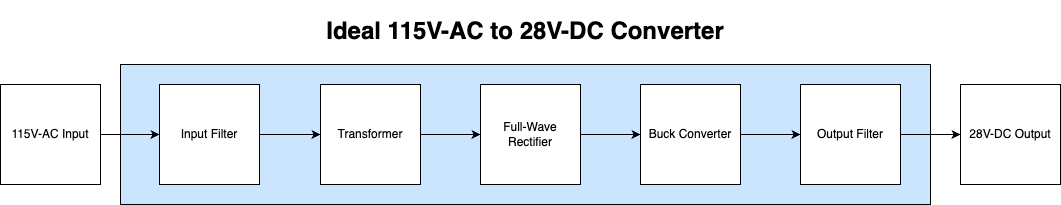
\includegraphics[width=1.0\linewidth]{ac_dc_converter_ideal.png}
    \caption{Ideal AC-DC Converter}
    \label{fig:ac_dc_converter_ideal_diagram}
\end{figure}

\begin{figure}[h]
    \centering
    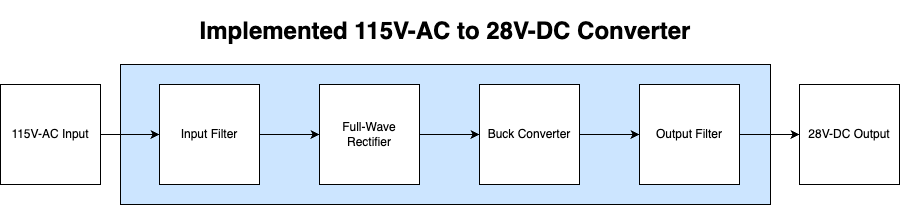
\includegraphics[width=1.0\linewidth]{ac_dc_converter_implemented.png}
    \caption{Implemented AC-DC Converter}
    \label{fig:ac_dc_converter_implemented_diagram}
\end{figure}

\subsection{Input Filter}

\subsection{Full-Wave Bridge Rectifier}
Directly after the AC input filters, the AC signal is fed into a full-wave bridge rectifier. The function of a full-wave rectifier is to convert both the positive and negative half cycles of an AC signal into a pulsating DC signal output, see Figure \ref{fig:full-wave_rectifier_output_waveform_diagram}. From there, a bulk capacitor is used on the output to "smooth" out the pulsating DC signal so that the output signal begins to resemble a stable DC output, see Figure \ref{fig:full-wave_bridge_rectifier_filter_waveform_diagram}. 

\begin{figure}[htp]
    \centering
    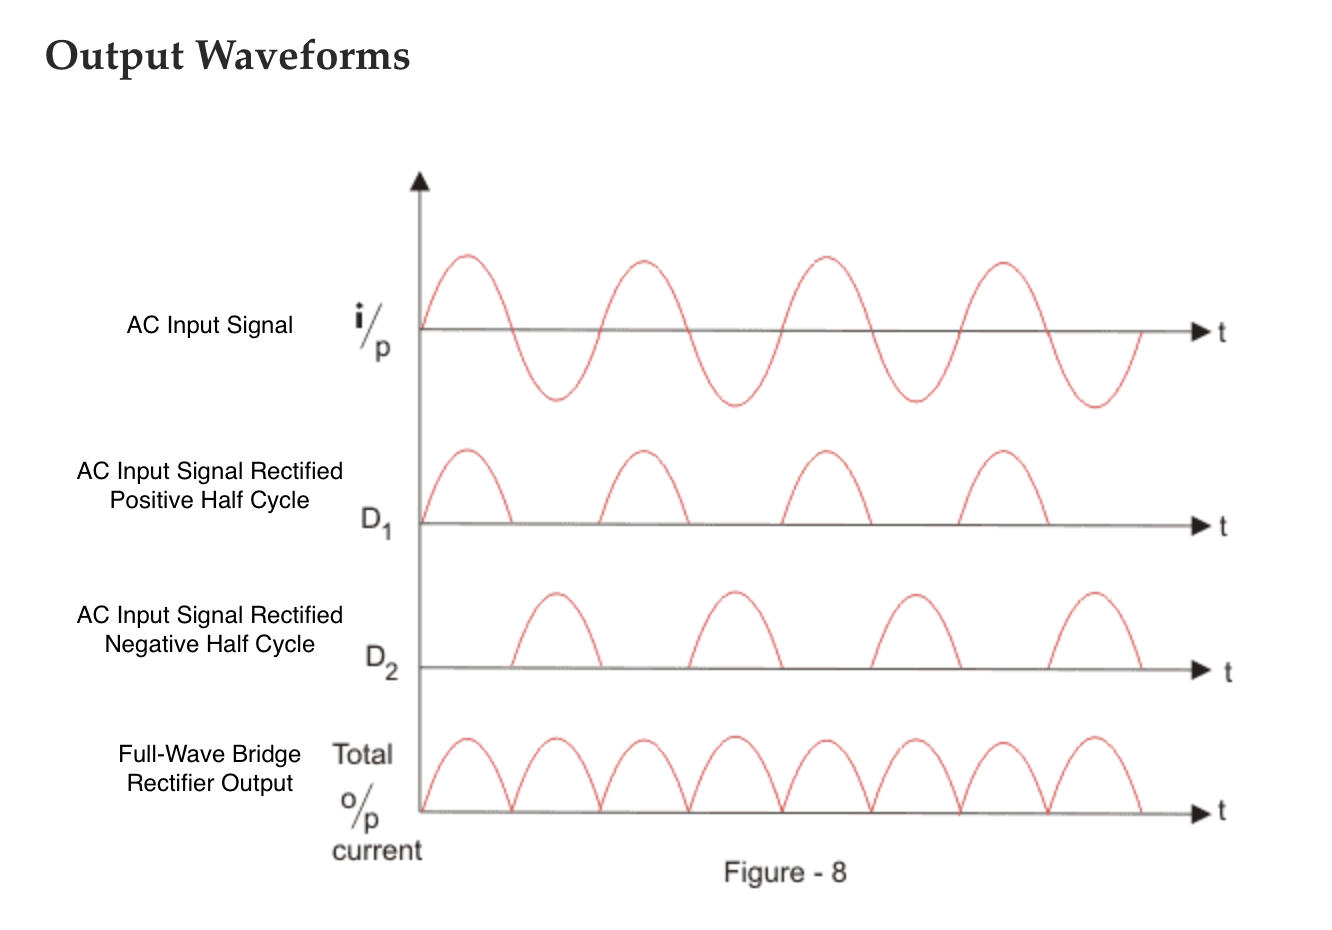
\includegraphics[width=1.0\linewidth]{full-wave_bridge_rectifier_output_waveform.png}
    \caption{Full-Wave Rectifier Output Waveforms}
    \label{fig:full-wave_rectifier_output_waveform_diagram}
\end{figure}

\begin{figure}[h]
    \centering
    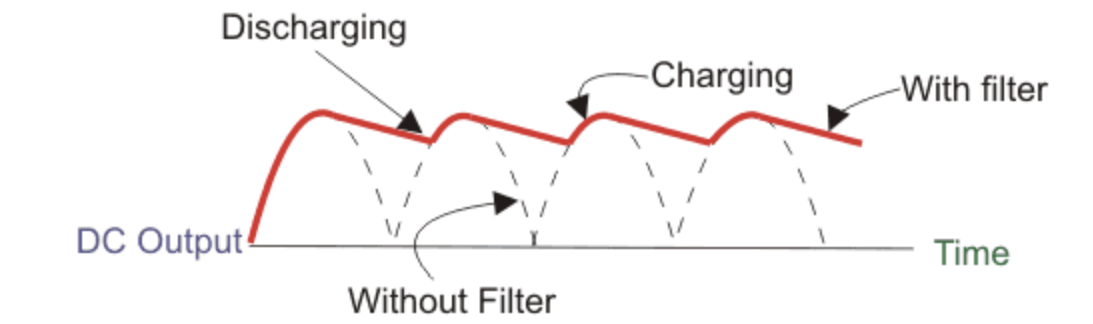
\includegraphics[width=1.0\linewidth]{full-wave_bridge_rectifier_filter_waveform.png}
    \caption{Full-Wave Rectifier Filter Waveform}
    \label{fig:full-wave_bridge_rectifier_filter_waveform_diagram}
\end{figure}


For our implementation, a full-wave bridge rectifier, see Figure \ref{fig:full-wave_bridge_rectifier_circuit_diagram} was implemented because it is more efficient than a half-wave rectifier. For a full-wave rectifier, both cycles of the AC signal are converted into the DC signal. For a half-wave rectifier, only a single half cycle of the AC signal is transferred, meanwhile the other half cycle is blocked. 

\begin{figure}[htp]
    \centering
    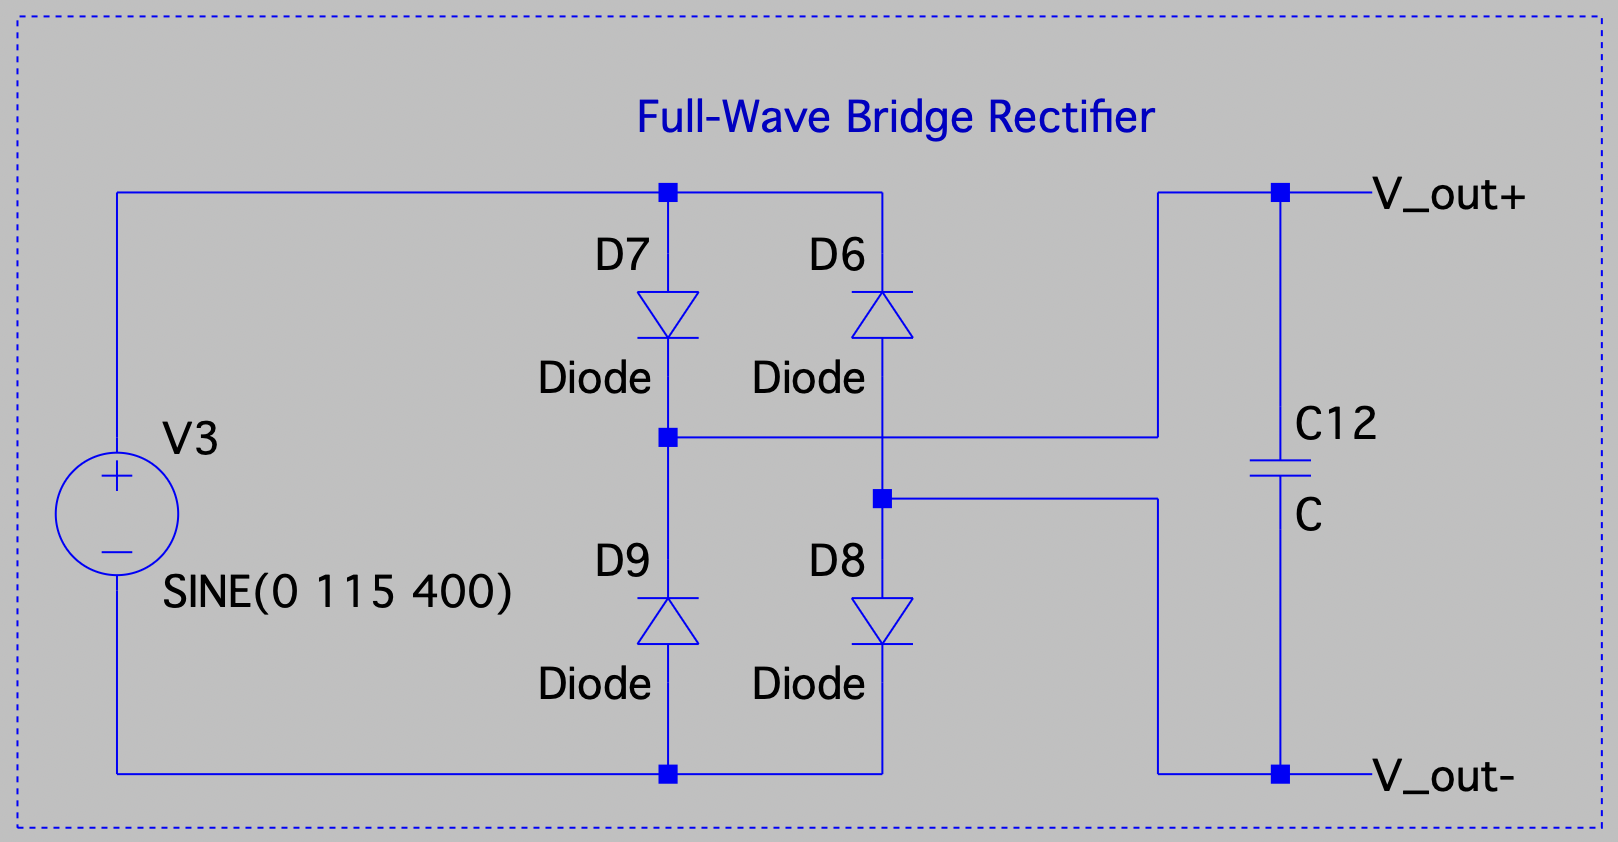
\includegraphics[width=1.0\linewidth]{full-wave_bridge_rectifier_circuit.png}
    \caption{Full-Wave Bridge Rectifier Circuit}
    \label{fig:full-wave_bridge_rectifier_circuit_diagram}
\end{figure}

To model the full-wave bridge rectifier in LTSpice

\subsection{Buck Converter}


\subsection{Output Filter}

\section{Simulation Setup}
\subsection{Input Filter}
\subsection{Full-Wave Bridge Rectifier}
\subsection{Buck Converter}
\subsection{Output Filter}


\section{Simulation Results}
\subsection{Input Filter}
\subsection{Full-Wave Bridge Rectifier}
\subsection{Buck Converter}
\subsection{Output Filter}
\subsection{Load}

\nocite{*}
\bibliographystyle{ieeetr}
\bibliography{final_project.bib}

\end{document}
